\documentclass[11pt]{article}
\usepackage{graphicx}
\graphicspath{ {./images/} }
\begin{document}
\title{Aplicaci\'on de algoritmo gen\'etico: N-queens }
\author{Orlando Hernandez Nu\~nez. Juan Alejandro Bernal Gallego}
\maketitle

\section{Introducci\'on}
En el presente trabajo se busca dar soluci\'on al problema de las N-queens mediante el uso de un algoritmo gen\'etico. A continuaci\'on, se mostrar\'a la configuraci\'on de par\'ametros con las que fue ejecutado el algoritmo gen\'etico y los resultados obtenidos.

\section{Problema}
En el juego de ajedrez la reina amenaza a aquellas piezas que se encuentren en su misma fila, columna o diagonal. El problema de las 8 reinas (o n-queens ya que dependen del numero asignado) consiste en poner sobre un tablero de ajedrez ocho reinas sin que estas se amenacen entre ellas.
\begin{figure}[h]
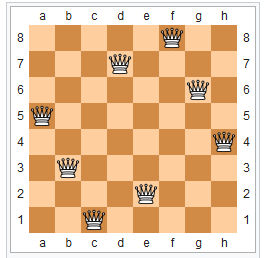
\includegraphics[width=8cm, height=6cm]{nqueens}
\centering
\caption{Soluci\'on al problema de las N-queens}
\end{figure}
\section{Algoritmo Gen\'etico}
\subsection{Definici\'on de la codificaci\'on}
Para representar cada uno de los cromosomas que integrar\'an la poblaci\'on de posibles soluciones
al problema se eligi\'o un vector de n\'umeros enteros donde cada indice indica una fila del tablero.
El valor de cada indice esta entre 0 y N-1 donde N es el n\'umero de reinas a distribuir en el tablero
y este valor indicar\'a en que columna se ubica la reina dentro del tablero.
\section{Codificación}
\label{sec:org3017964}
\subsection{Lógica}
\label{sec:org7b5bbe9}
Los cromosomas fueron codificados de manera que pudieran representar la ubicación en columnas y filas de cada columna. El gen representa la columna en la que se encuentra cada reina, y el indice del gen representa la posición de las reinas con respecto a las filas.
\begin{itemize}
\item Ejemplo: Cromosoma 1 = \{1, 2, 0\} seria las posiciones de 3 reinas en un tablero de 3x3
0 1 0
0 0 1
1 0 0
\end{itemize}

\subsection{Modelo}
\label{sec:org9bc4bf7}
El modelo utilizado para representar cada posible solución es de lograr alcanzar un cromosoma que tenga 0 cruces, en el ejemplo anterior se puede apreciar que hay un cruces entre el gen 0 y el gen 1, esto genera un cruce total de 2 para este cromosoma, luego en la función de fitness mostramos como utilizamos estos cruces para conseguir alcanzar un fitness que represente correctamente el objetivo deseado (minimizar cruces)
\end{document}
